\documentclass[10pt,a4paper]{article}
\usepackage[utf8]{inputenc}
\usepackage{amsthm, amsmath, mathtools, amssymb}
\usepackage[left=2cm,right=2cm,top=2cm,bottom=2cm]{geometry}
\usepackage[colorlinks,linkcolor=blue,citecolor=blue,urlcolor=blue]{hyperref}
\usepackage[catalan]{babel}
\usepackage{titlesec}
\usepackage{enumitem}
\usepackage{physics}
\usepackage{fancyhdr}
\usepackage{subcaption}
\usepackage{xcolor}
\usepackage{listings} 
\usepackage{parskip} % exchanges indentation for spacing between paragraphs.
\usepackage{hyperref} % link automatically references.
% \usepackage{hycolor} % implements options of colors for hyperref (it ables the user to use colors from xcolor package)
\usepackage[capitalise,nameinlink]{cleveref}

\definecolor{darkblue}{rgb}{0.0, 0.0, 0.55}

  \lstloadlanguages{C,Python,bash}
  \lstset{ %
          backgroundcolor=\color{white},   % choose the background color; you must add \usepackage{color} or \usepackage{xcolor}
          basicstyle=\color{red}\footnotesize\ttfamily,        % the size of the fonts that are used for the code
          breakatwhitespace=false,         % sets if automatic breaks should only happen at whitespace
          breaklines=true,                 % sets automatic line breaking
          captionpos=b,                    % sets the caption-position to bottom
          deletekeywords={...},            % if you want to delete keywords from the given language
          escapeinside={\%*}{*)},          % if you want to add LaTeX within your code
          extendedchars=true,              % lets you use non-ASCII characters; for 8-bits encodings only, does not work with UTF-8
          frame=single,                    % adds a frame around the code
          keepspaces=true,                 % keeps spaces in text, useful for keeping indentation of code (possibly needs columns=flexible)
          keywordstyle=\color{darkblue},       % keyword style
          commentstyle=\itshape\color{gray},
          identifierstyle=\color{black},
          language=C,                 % the language of the code
          otherkeywords={*,...},           % if you want to add more keywords to the set
          numbers=left,                    % where to put the line-numbers; possible values are (none, left, right)
          numbersep=5pt,                   % how far the line-numbers are from the code
          numberstyle=\tiny\color{gray}, % the style that is used for the line-numbers
          rulecolor=\color{gray},         % if not set, the frame-color may be changed on line-breaks within not-black text (e.g. comments (green here))
          showspaces=false,                % show spaces everywhere adding particular underscores; it overrides 'showstringspaces'
          showstringspaces=false,          % underline spaces within strings only
          showtabs=false,                  % show tabs within strings adding particular underscores
          stepnumber=1,                    % the step between two line-numbers. If it's 1, each line will be numbered
          stringstyle=\color{blue},     % string literal style
          tabsize=2,                         % sets default tabsize to 2 spaces
          %title=\lstname                   % show the filename of files included with \lstinputlisting; also try caption instead of title
  }
  \lstset{literate=
          {á}{{\'a}}1 {é}{{\'e}}1 {í}{{\'i}}1 {ó}{{\'o}}1 {ú}{{\'u}}1
          {Á}{{\'A}}1 {É}{{\'E}}1 {Í}{{\'I}}1 {Ó}{{\'O}}1 {Ú}{{\'U}}1
          {à}{{\`a}}1 {è}{{\`e}}1 {ì}{{\`i}}1 {ò}{{\`o}}1 {ù}{{\`u}}1
          {À}{{\`A}}1 {È}{{\'E}}1 {Ì}{{\`I}}1 {Ò}{{\`O}}1 {Ù}{{\`U}}1
          {ä}{{\"a}}1 {ë}{{\"e}}1 {ï}{{\"i}}1 {ö}{{\"o}}1 {ü}{{\"u}}1
          {Ä}{{\"A}}1 {Ë}{{\"E}}1 {Ï}{{\"I}}1 {Ö}{{\"O}}1 {Ü}{{\"U}}1
          {â}{{\^a}}1 {ê}{{\^e}}1 {î}{{\^i}}1 {ô}{{\^o}}1 {û}{{\^u}}1
          {Â}{{\^A}}1 {Ê}{{\^E}}1 {Î}{{\^I}}1 {Ô}{{\^O}}1 {Û}{{\^U}}1
          {œ}{{\oe}}1 {Œ}{{\OE}}1 {æ}{{\ae}}1 {Æ}{{\AE}}1 {ß}{{\ss}}1
          {ű}{{\H{u}}}1 {Ű}{{\H{U}}}1 {ő}{{\H{o}}}1 {Ő}{{\H{O}}}1
          {ç}{{\c c}}1 {Ç}{{\c C}}1 {ø}{{\o}}1 {å}{{\r a}}1 {Å}{{\r A}}1
          {€}{{\EUR}}1 {£}{{\pounds}}1
  }




\newcommand{\NN}{\ensuremath{\mathbb{N}}} % set of natural numbers
\newcommand{\ZZ}{\ensuremath{\mathbb{Z}}} % set of integers
\newcommand{\QQ}{\ensuremath{\mathbb{Q}}} % set of rationals
\newcommand{\RR}{\ensuremath{\mathbb{R}}} % set of real numbers
\newcommand{\CC}{\ensuremath{\mathbb{C}}} % set of complex numbers
\newcommand{\KK}{\ensuremath{\mathbb{K}}} % a general field

\newcommand{\vf}[1]{\boldsymbol{\mathrm{#1}}} % math style for vectors and matrices and vector-values functions (previously it was \*vb{#1} but this does not apply to greek letters)
\newcommand{\ii}{\mathrm{i}} % imaginary unit
\renewcommand{\O}{\mathrm{O}} % big O-notation

\newtheorem{theorem}{Teorema}
\newtheorem{exercici}{Exercise}
\newtheorem{prop}{Proposició}
\theoremstyle{definition}
\newtheorem{definition}{Definició}
\theoremstyle{remark}
\newtheorem*{res}{Resolution}
\DeclareDocumentCommand\derivative{ s o m g d() }{ 
  % Total derivative
  % s: star for \flatfrac flat derivative
  % o: optional n for nth derivative
  % m: mandatory (x in df/dx)
  % g: optional (f in df/dx)
  % d: long-form d/dx(...)
    \IfBooleanTF{#1}
    {\let\fractype\flatfrac}
    {\let\fractype\frac}
    \IfNoValueTF{#4}
    {
        \IfNoValueTF{#5}
        {\fractype{\diffd \IfNoValueTF{#2}{}{^{#2}}}{\diffd #3\IfNoValueTF{#2}{}{^{#2}}}}
        {\fractype{\diffd \IfNoValueTF{#2}{}{^{#2}}}{\diffd #3\IfNoValueTF{#2}{}{^{#2}}} \argopen(#5\argclose)}
    }
    {\fractype{\diffd \IfNoValueTF{#2}{}{^{#2}} #3}{\diffd #4\IfNoValueTF{#2}{}{^{#2}}}\IfValueT{#5}{(#5)}}
} % differential operator
\DeclareDocumentCommand\partialderivative{ s o m g d() }{ 
  % Total derivative
  % s: star for \flatfrac flat derivative
  % o: optional n for nth derivative
  % m: mandatory (x in df/dx)
  % g: optional (f in df/dx)
  % d: long-form d/dx(...)
  \IfBooleanTF{#1}
    {\let\fractype\flatfrac}
    {\let\fractype\frac}
    \IfNoValueTF{#4}{
      \IfNoValueTF{#5}
      {\fractype{\partial \IfNoValueTF{#2}{}{^{#2}}}{\partial #3\IfNoValueTF{#2}{}{^{#2}}}}
      {\fractype{\partial \IfNoValueTF{#2}{}{^{#2}}}{\partial #3\IfNoValueTF{#2}{}{^{#2}}} \argopen(#5\argclose)}
    }
    {\fractype{\partial \IfNoValueTF{#2}{}{^{#2}} #3}{\partial #4\IfNoValueTF{#2}{}{^{#2}}}\IfValueT{#5}{(#5)}}
} % partial differential operator

\titleformat{\section}
  {\normalfont\fontsize{11}{15}\bfseries}{\thesection}{1em}{}

% \renewcommand{\theenumi}{\textbf{\arabic{enumi}}}
\renewcommand{\theenumi}{\alph{enumi}}
\renewcommand{\theenumiii}{\roman{enumiii}}
\renewcommand{\exp}[1]{\mathrm{e}^{#1}} % exponential function
\DeclareMathOperator*{\im}{Im}

\title{\bfseries\Large Octave problems}

\author{Víctor Ballester Ribó\\NIU: 1570866}
\date{\parbox{\linewidth}{\centering
  Integració numèrica d'equacions en derivades parcials\endgraf
  Grau en Matemàtiques\endgraf
  Universitat Autònoma de Barcelona\endgraf
  Juny de 2023}}
  \pagestyle{fancy}
  \fancyhf{}
  \fancyhfoffset[L]{1cm}
  \fancyhfoffset[R]{1cm}
  \rhead{NIU: 1570866}
  \lhead{Víctor Ballester}
  \cfoot{\thepage}
  %\setlength{\headheight}{13.6pt}

\setlength{\parindent}{0pt}
\begin{document}
\selectlanguage{catalan}
\maketitle
\setcounter{exercici}{2}
\begin{exercici}
  For values of $x\in[-1,3]$ and $t\in [0,2.4]$, compare the following numerical schemes for the one-dimensional wave equation
  $$
    u_t+u_x=0
  $$
  with initial condition
  $$
    u(0,x)=\begin{cases}
      {\cos(\pi x)}^2 & \abs{x}\leq \frac{1}{2} \\
      0               & \text{otherwise}
    \end{cases}
  $$
  and boundary condition $u(t,-1)=0$. Use spatial time steps of $h=1/10$, $h=1/20$, and $h=1/40$.
  \begin{enumerate}
    \item Forward-time, backward-space (FTBS) with $\lambda =0.8$.
          \item\label{ex1:b} Forward-time, centered-space (FTCS) with $\lambda =0.8$.
          \item\label{ex1:c} Lax-Friedrichs (LF) with $\lambda =0.8$ and $\lambda =1.6$.
          \item\label{ex1:d} Leapfrog (L) with $\lambda =0.8$ and using the forward-time, centered-space scheme for the first step.
  \end{enumerate}
  For the schemes \ref{ex1:b}, \ref{ex1:c}, and \ref{ex1:d}, use the numerical boundary condition $v_M^{n+1}=v_{M-1}^{n+1}$.
\end{exercici}
\begin{res}
  In the next table we expose the error in $L^2$ norm of all the experiments that we have done.
  \begin{table}[ht]
    \centering
    \begin{tabular}{|l|c|c|c|}
      \hline
      Scheme               & $h=1/10$ & $h=1/20$  & $h=1/40$             \\
      \hline\hline
      FTBS ($\lambda=0.8$) & 0.192501 & 0.119992  & 0.068666             \\
      FTCS ($\lambda=0.8$) & 26.0543  & 4337.15   & $1.63829\times 10^9$ \\
      LF ($\lambda=0.8$)   & 0.293134 & 0.206742  & 0.130863             \\
      LF ($\lambda=1.6$)   & 22.6263  & 2274.83   & $4.01576\times 10^8$ \\
      L ($\lambda=0.8$)    & 0.163822 & 0.0417945 & 0.0114763            \\
      \hline
    \end{tabular}
    \caption{Error in $L^2$ norm for the different schemes.}
  \end{table}

  From here we can conclude that the useful schemes are the FTBS with $\lambda=0.8$, the Lax-Friedrichs with $\lambda=0.8$ and the Leapfrog with $\lambda=0.8$. And the other ones are useless as the error seams to approach to infinity as we decrease the step size $h$. In \cref{fig:convergent1} we show the solutions of the three convergent methods with the three spatial steps mentioned above.
  \begin{figure}[ht]
    \centering
    \begin{subfigure}{0.49\textwidth}
      \centering
      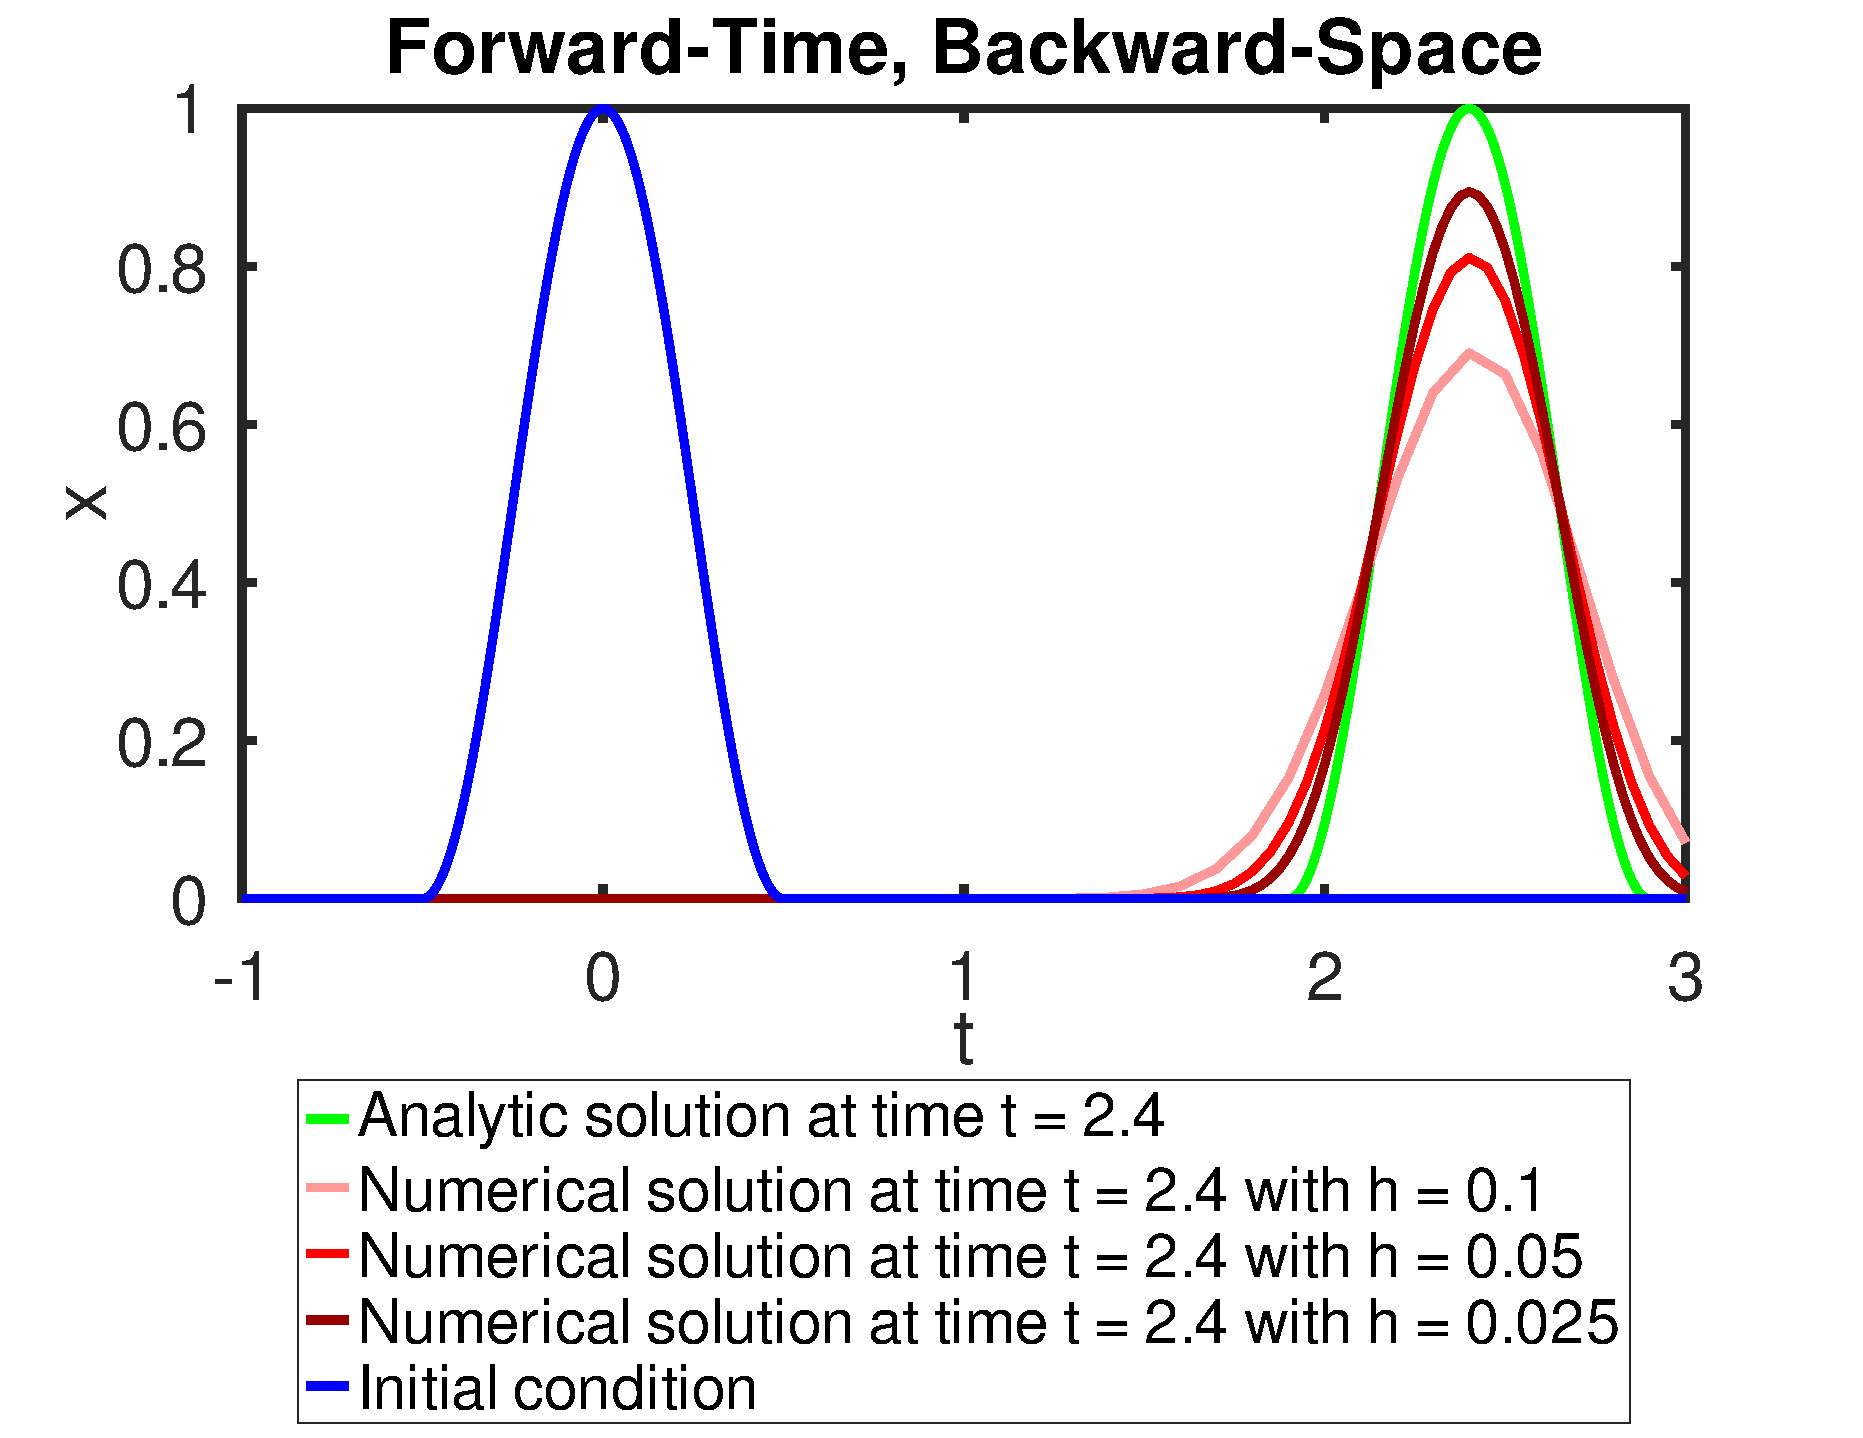
\includegraphics[width=\textwidth]{Images/ftbs.pdf}
      \caption{FTBS with $\lambda=0.8$.}
    \end{subfigure}\hfill
    \begin{subfigure}{0.49\textwidth}
      \centering
      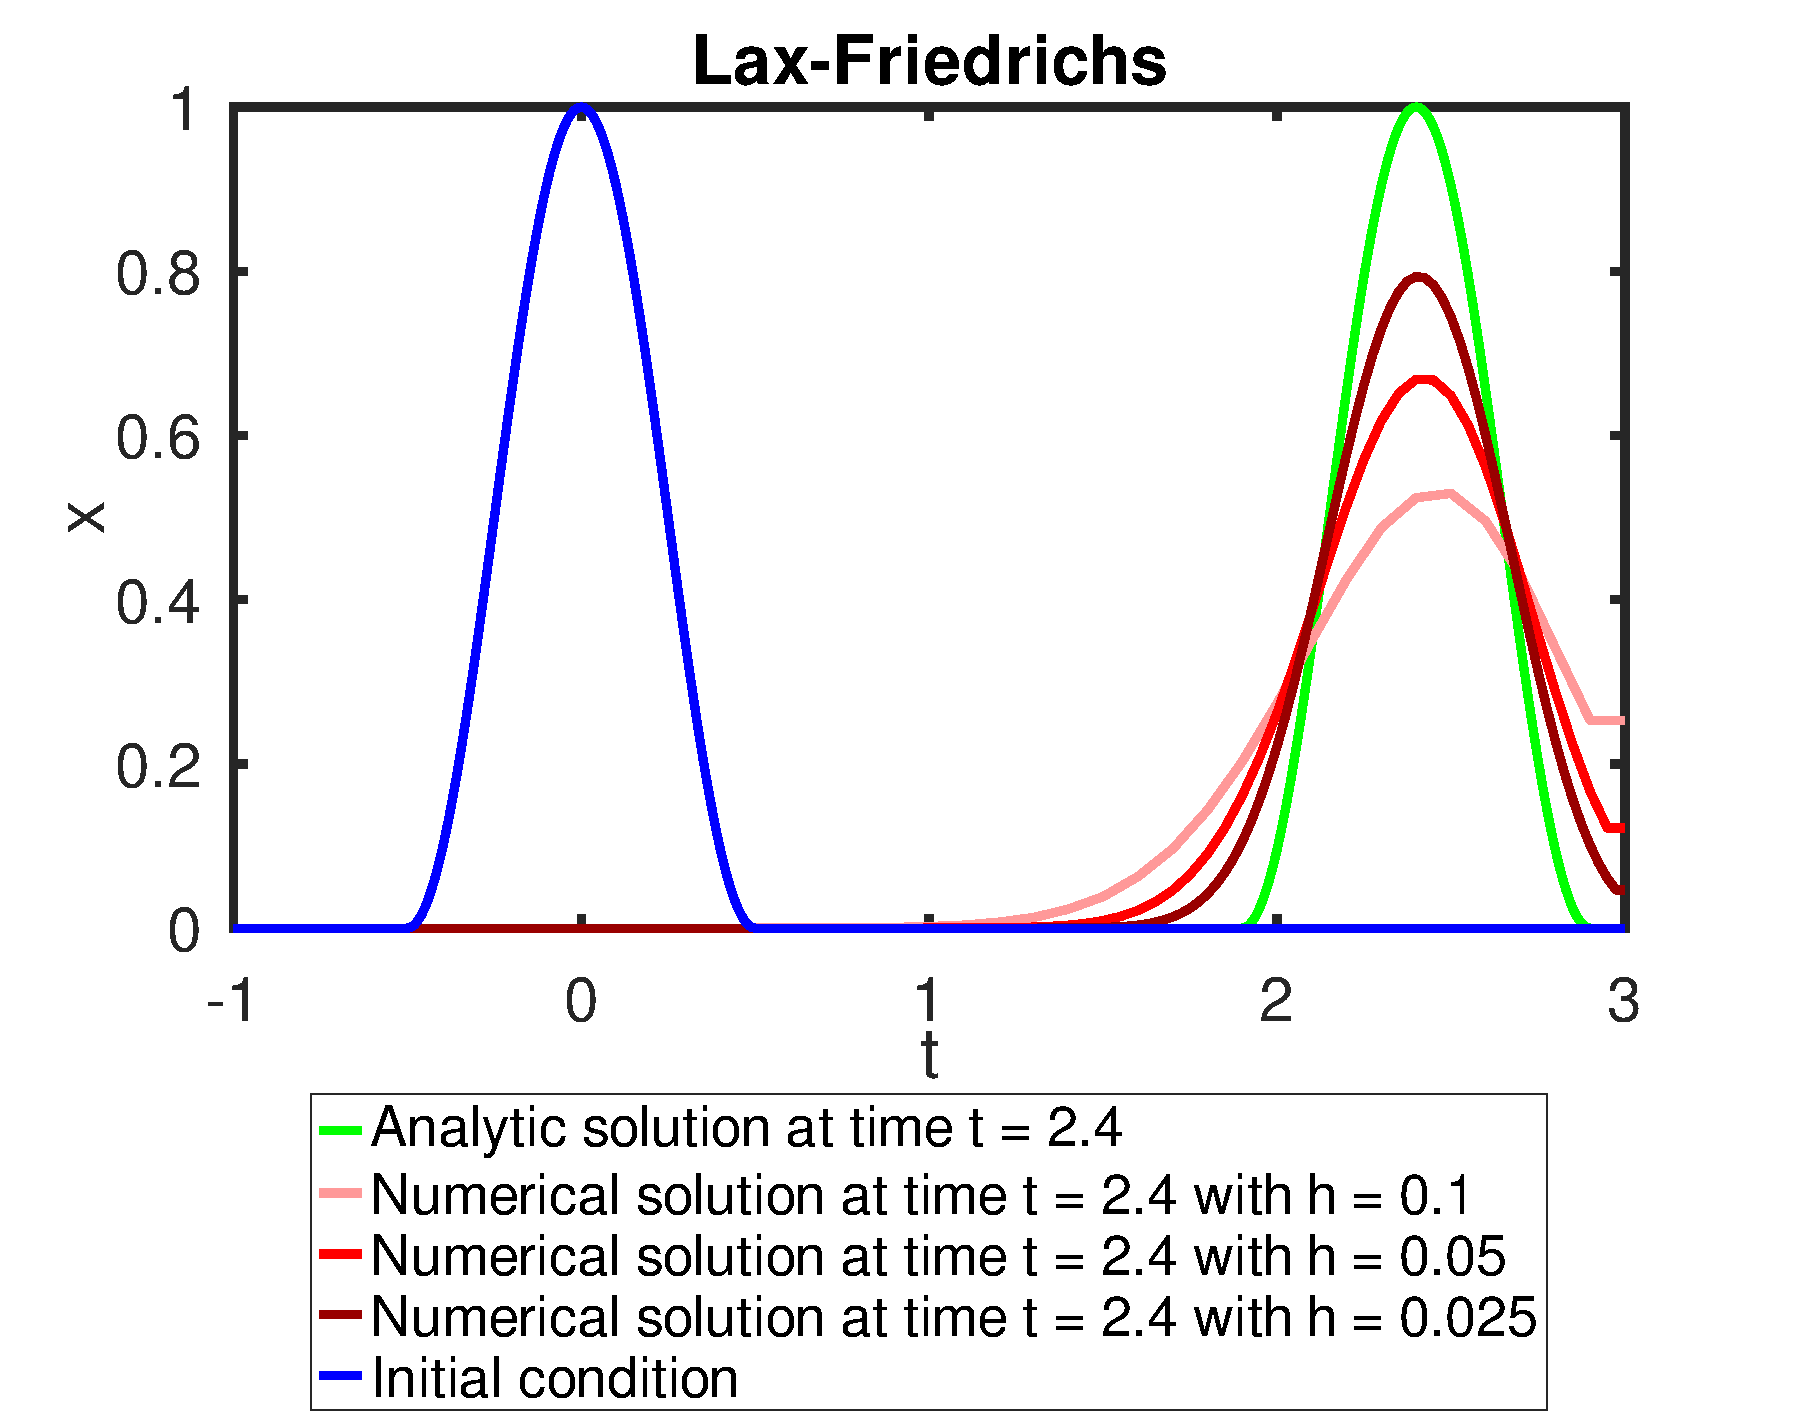
\includegraphics[width=\textwidth]{Images/lf.pdf}
      \caption{Lax-Friedrichs with $\lambda=0.8$.}
    \end{subfigure}\hfill
    \begin{subfigure}{0.49\textwidth}
      \centering
      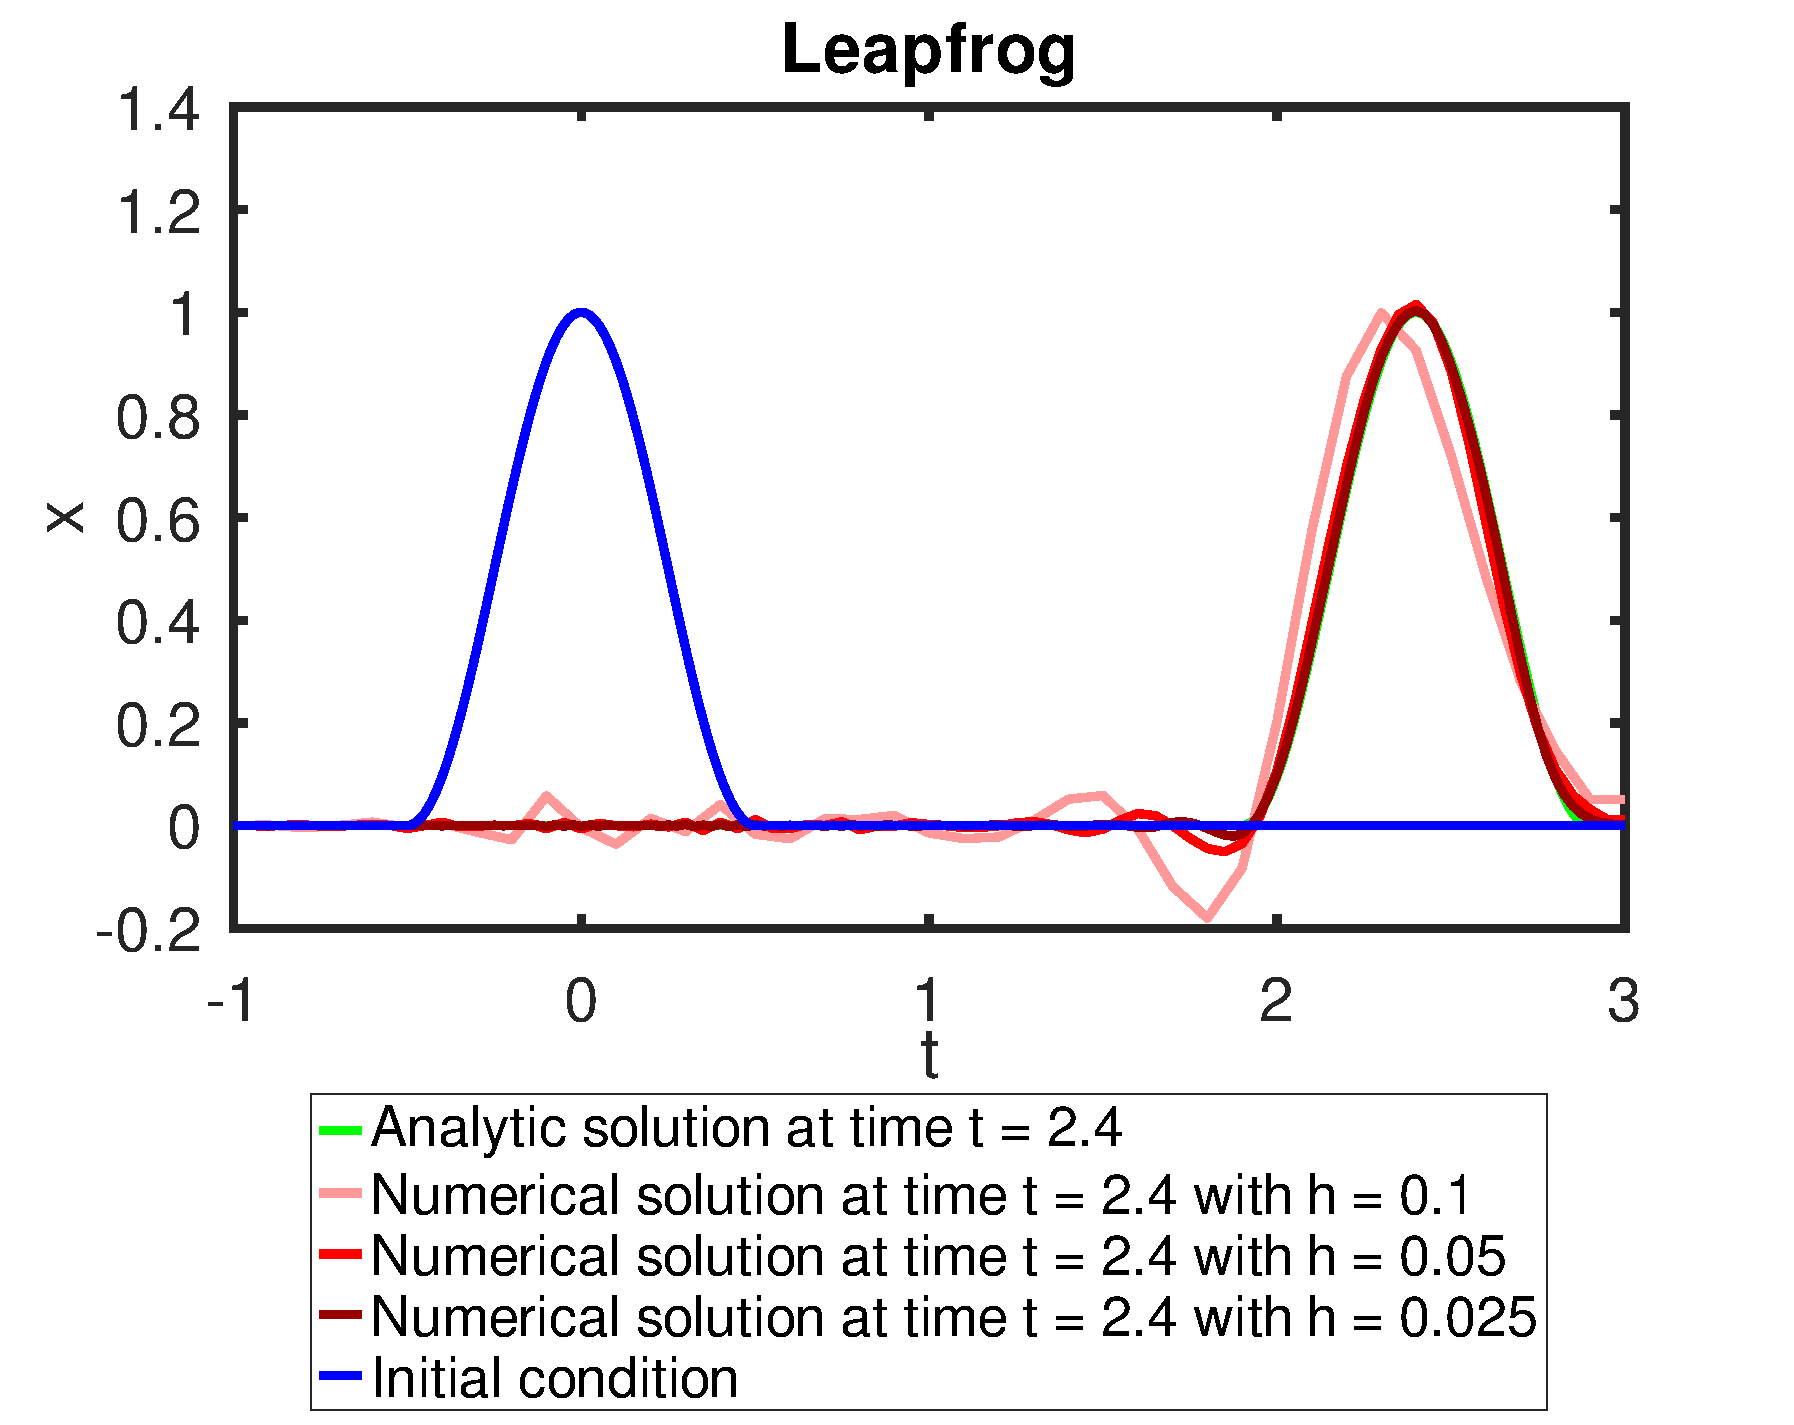
\includegraphics[width=\textwidth]{Images/l.pdf}
      \caption{Leapfrog with $\lambda=0.8$.}
    \end{subfigure}
    \caption{Plot of the analytical and numerical solutions of the convergent schemes}
    \label{fig:convergent1}
  \end{figure}
  \newpage
  We can do now a further analysis of these three schemes. In the following table we summarize the error and order of convergence of these schemes as we halve the step size $h$.

  \begin{table}[!ht]
    \centering
    \begin{tabular}{|c||c|c|c||c|c|c||c|c|c|}
      \hline
              & \multicolumn{3}{c||}{FTBS} & \multicolumn{3}{c||}{Lax-Friedrichs} & \multicolumn{3}{c|}{Leapfrog}                                                                                \\
      \cline{2-10}
      $h$     & Error                      & Rate                                 & Order                         & Error       & Rate      & Order      & Error         & Rate      & Order     \\
      \hline\hline
      $1/10$  & $0.192501$                 & -                                    & -                             & $0.293134$  & -         & -          & $0.163822$    & -         & -         \\
      $1/20$  & $0.119992$                 & $1.60429$                            & $0.681933$                    & $0.206742$  & $1.41787$ & $0.50373$  & $0.0417945$   & $3.9197$  & $1.97074$ \\
      $1/40$  & $0.068666$                 & $1.74747$                            & $0.805267$                    & $0.130863$  & $1.57984$ & $0.659776$ & $0.0114763$   & $3.64181$ & $1.86466$ \\
      $1/80$  & $0.0371725$                & $1.84723$                            & $0.88536$                     & $0.0758213$ & $1.72593$ & $0.787377$ & $0.00324644$  & $3.53504$ & $1.82172$ \\
      $1/160$ & $0.0194683$                & $1.90939$                            & $0.93311$                     & $0.0413688$ & $1.83281$ & $0.87406$  & $0.000942768$ & $3.44352$ & $1.78388$ \\
      $1/320$ & $0.0100036$                & $1.94612$                            & $0.960603$                    & $0.0217645$ & $1.90075$ & $0.926566$ & $0.00027973$  & $3.37028$ & $1.75287$ \\
      \hline
    \end{tabular}
    \caption{Errors in norm $L^2$ and orders for the three schemes.}
  \end{table}

  The values in both tables were obtained executing:
  \begin{lstlisting}[language=Matlab]
getResults
\end{lstlisting}
  Observe that the forward-time, backward-space and the Lax-Friedrichs schemes converge as approximately a first-order scheme, whereas the Leapfrog method as a second-order scheme. An interesting fact to note here is that the Leapfrog \emph{loses} convergency as we decrease the stepsize. This is not strange, as it may happen that the numerical order of convergency differ from the theoretical order of convergency, because of propagation of errors.

  We add here the plots of the divergent schmes. Observe the oscillating pattern.
  \begin{figure}[ht]
    \centering
    \begin{subfigure}{0.49\textwidth}
      \centering
      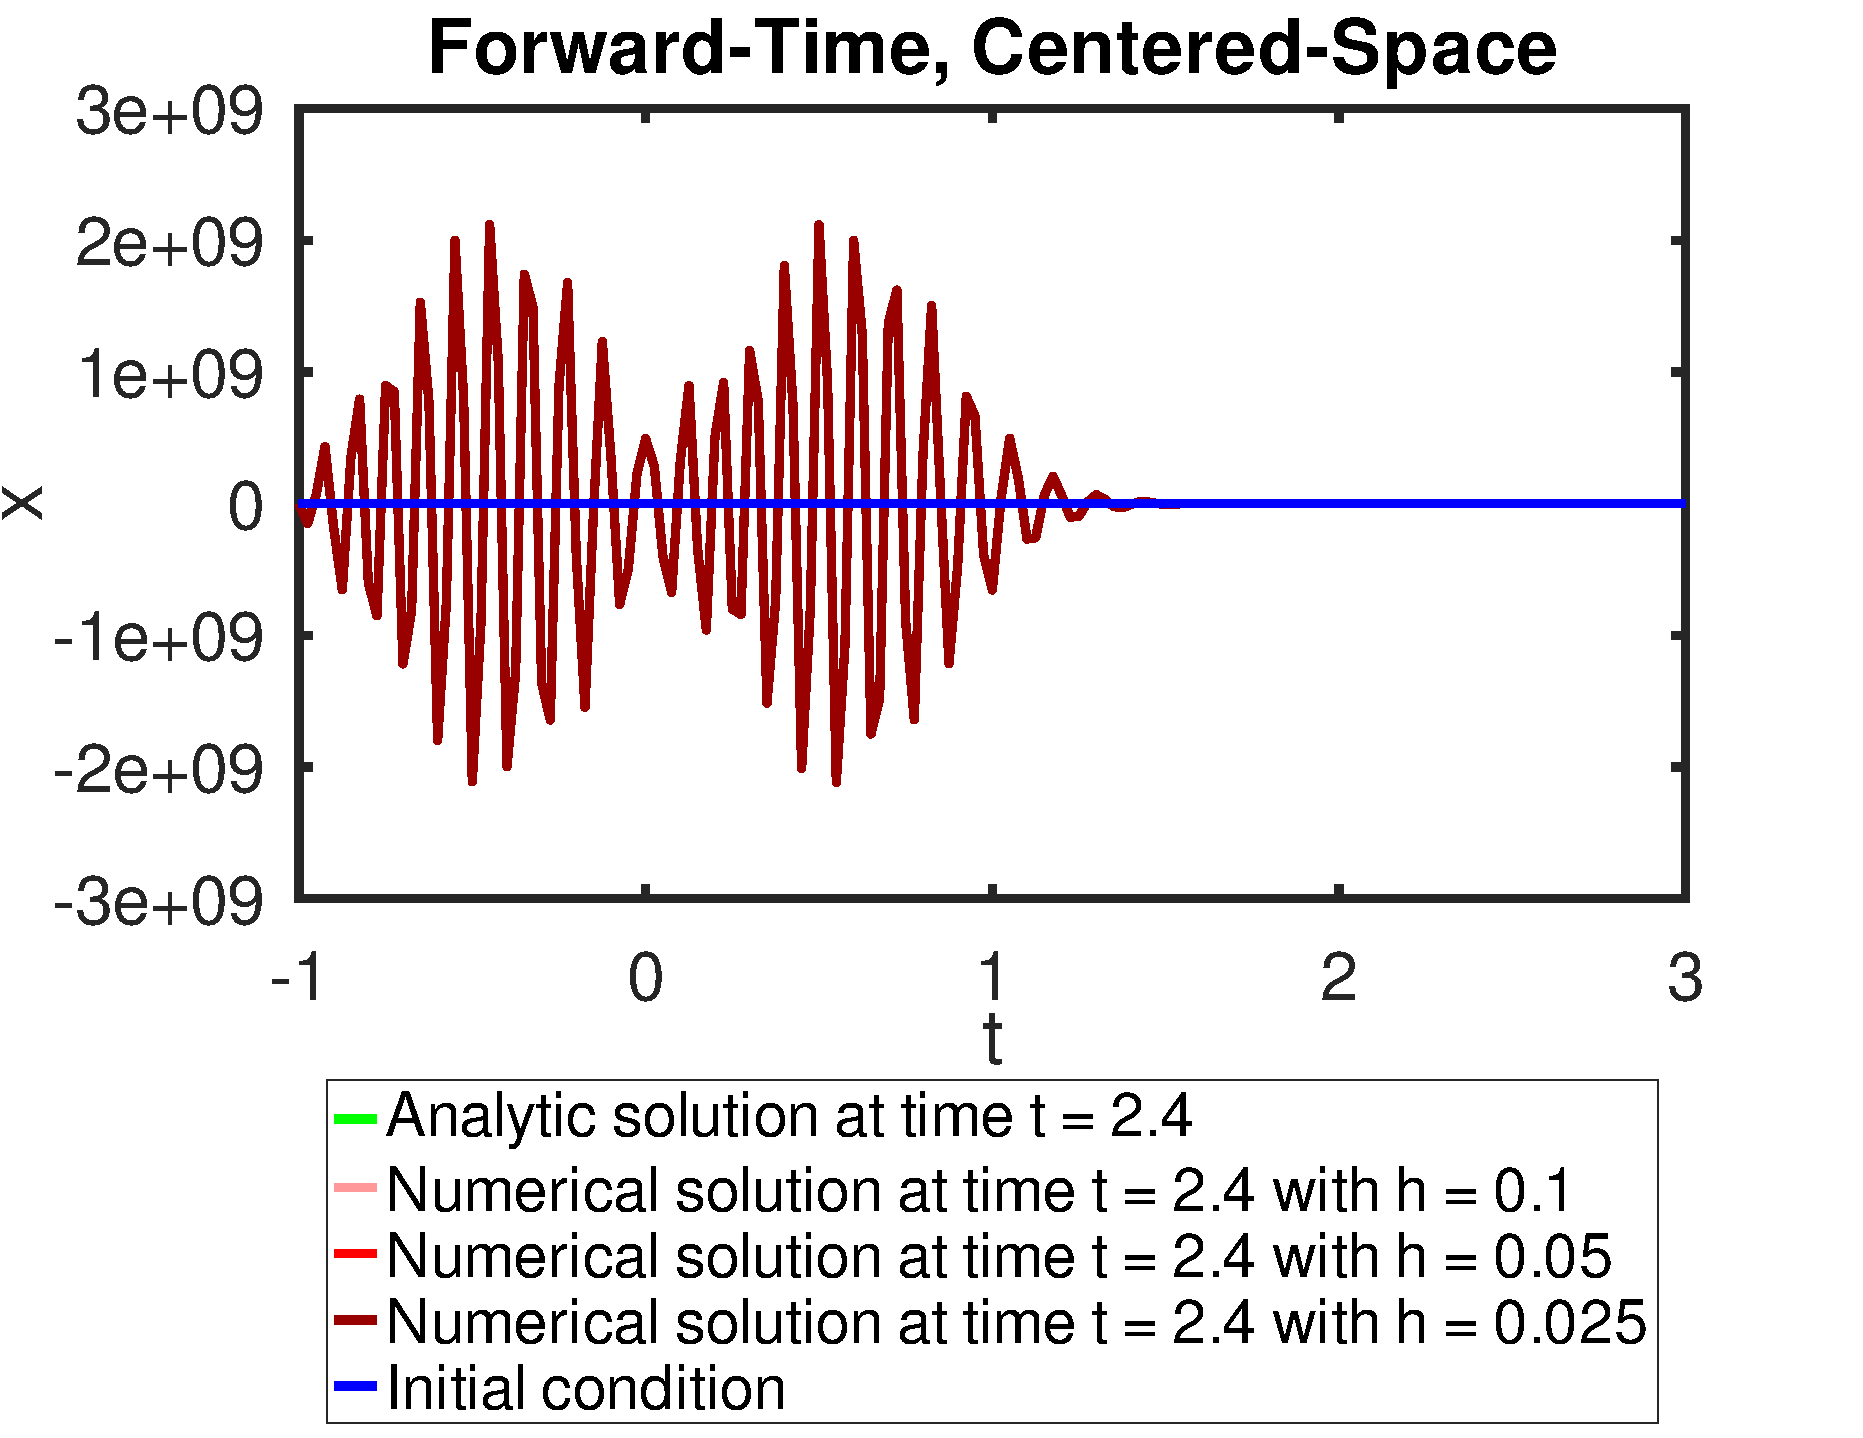
\includegraphics[width=\textwidth]{Images/ftcs.pdf}
      \caption{FTCS with $\lambda=0.8$.}
    \end{subfigure}\hfill
    \begin{subfigure}{0.49\textwidth}
      \centering
      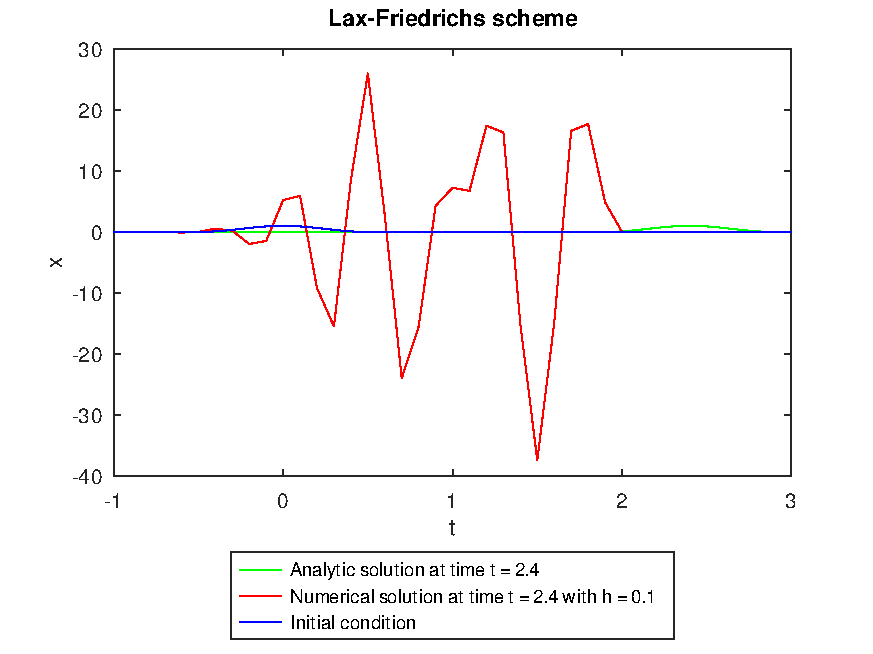
\includegraphics[width=\textwidth]{Images/lf_div.pdf}
      \caption{Lax-Friedrichs with $\lambda=1.6$.}
    \end{subfigure}
    \caption{Plot of the analytical and numerical solutions of the divergent schemes}
  \end{figure}
\end{res}
\newpage
\setcounter{exercici}{14}
\begin{exercici}
  Solve $u_t+u_x=0$, $x\in[-1,1]$, $t\in[0,1.2]$, with initial condition $u(0,x)=\sin(2\pi x)$ and periodicity $u(t,-1)=u(t,1)$. Use the following schemes:
  \begin{enumerate}
    \item Forward-time, backward-space (FTBS) with $\lambda =0.8$.
    \item Lax-Wendroff (LW) with $\lambda =0.8$.
  \end{enumerate}
  Demonstrate the first-order accuracy of the FTBS scheme and the second-order accuracy of the LW scheme using time steps of $h=1/10$, $h=1/20$, $h=1/40$ and $h=1/80$. Do it in both the norm $L^2$ and the norm $L^\infty$.
\end{exercici}
\begin{res}
  The next tables summarize all the experiments that we have done. Note that we obtain a first order of approximation with the FTBS scheme and a second order of approximation with the Lax-Wendroff scheme, in both $L^2$ and $L^\infty$ norms.
  \begin{table}[ht]
    \centering
    \begin{tabular}{|c||c|c|c|c|c|c|}
      \hline
             & \multicolumn{6}{c|}{Forward-time, backward-space}                                                                              \\
      \cline{2-7}
             & \multicolumn{3}{c|}{$L^2$}                        & \multicolumn{3}{c|}{$L^\infty$}                                            \\
      \cline{2-7}
      $h$    & Error                                             & Rate                            & Order    & Error    & Rate    & Order    \\
      \hline\hline
      $1/10$ & 0.379872                                          & -                               & -        & 0.371158 & -       & -        \\
      $1/20$ & 0.211259                                          & 1.79813                         & 0.846501 & 0.371158 & 1.75963 & 0.815271 \\
      $1/40$ & 0.111737                                          & 1.89068                         & 0.918907 & 0.21093  & 1.88856 & 0.917286 \\
      $1/80$ & 0.0575043                                         & 1.94311                         & 0.958366 & 0.111688 & 1.94248 & 0.957901 \\
      \hline
    \end{tabular}
    \caption{Errors and orders for the FTBS scheme.}
  \end{table}\vspace{-0.4cm}
  \begin{table}[ht]
    \centering
    \begin{tabular}{|c||c|c|c|c|c|c|}
      \hline
             & \multicolumn{6}{c|}{Lax-Wendroff}                                                                             \\
      \cline{2-7}
             & \multicolumn{3}{c|}{$L^2$}        & \multicolumn{3}{c|}{$L^\infty$}                                           \\
      \cline{2-7}
      $h$    & Error                             & Rate                            & Order   & Error     & Rate    & Order   \\
      \hline\hline
      $1/10$ & 0.169042                          & -                               & -       & 0.166403  & -       & -       \\
      $1/20$ & 0.0441959                         & 3.82482                         & 1.93539 & 0.166403  & 3.78585 & 1.92062 \\
      $1/40$ & 0.0111394                         & 3.96753                         & 1.98824 & 0.0439539 & 3.95231 & 1.9827  \\
      $1/80$ & 0.00278932                        & 3.9936                          & 1.99769 & 0.0111211 & 3.98882 & 1.99596 \\
      \hline
    \end{tabular}
    \caption{Errors and orders for the Lax-Wendroff scheme.}
  \end{table}

  These values were obtained executing:
  \begin{lstlisting}[language=Matlab]
getResults
\end{lstlisting}
  \begin{figure}[!ht]
    \centering
    \begin{subfigure}{0.49\textwidth}
      \centering
      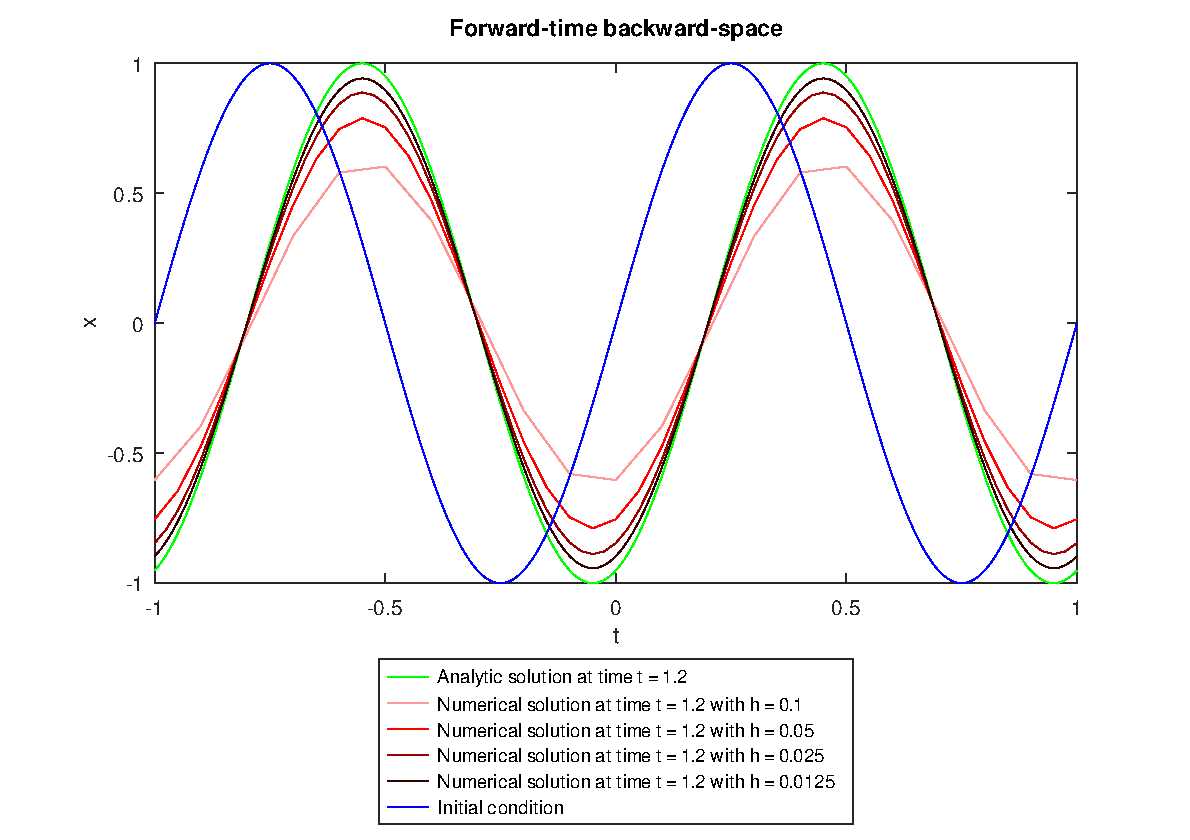
\includegraphics[width=\textwidth]{Images/ex2-ftbs.pdf}
      \caption{FTBS with $\lambda=0.8$.}
    \end{subfigure}\hfill
    \begin{subfigure}{0.49\textwidth}
      \centering
      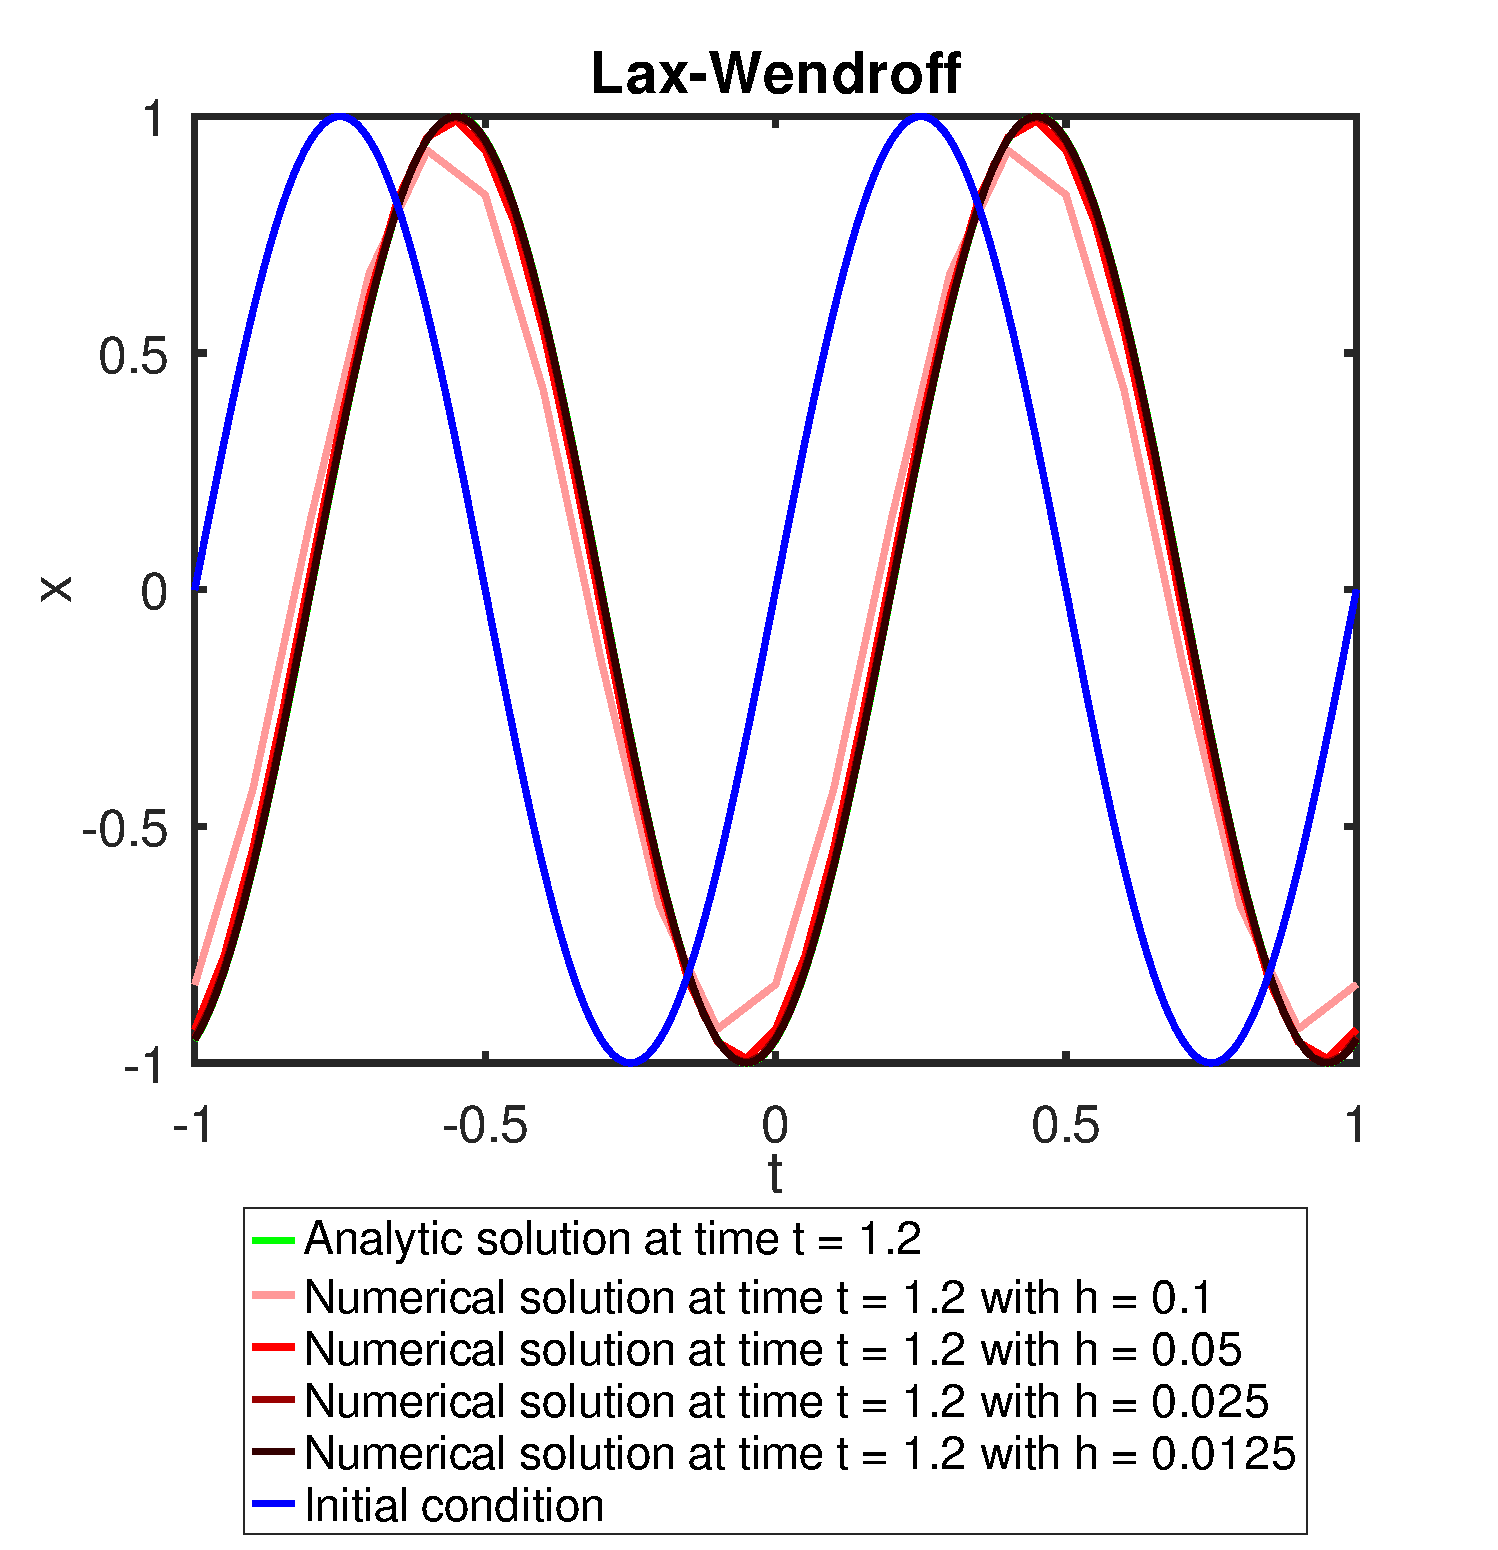
\includegraphics[width=\textwidth]{Images/ex2-lw.pdf}
      \caption{Lax-Wendroff with $\lambda=0.8$.}
    \end{subfigure}
    \caption{Plot of the analytical and numerical solutions of the FTBS and Lax-Wendroff schemes}
  \end{figure}

  To get the previous plots, execute the following commands:
  \begin{lstlisting}[language=Matlab]
a=1;x0=-1;x1=1;t1=1.2;lamb=0.8;myplot(a,lamb,0.01,x0,x1,t1,@ftbs,"Forward-Time, Backward-Space");
a=1;x0=-1;x1=1;t1=1.2;lamb=0.8;myplot(a,lamb,0.01,x0,x1,t1,@lw,"Lax-Wendroff");
\end{lstlisting}
\end{res}
\newpage
\setcounter{exercici}{27}
\begin{exercici}
  For a Dirichlet problem in the unit square with homogeneous boundary conditions, experimentally verify that:
  \begin{enumerate}
    \item The second-order finite difference discretization of the Poisson equation leads to a globally convergent scheme with quadratic error in the step size.
    \item The discretization using the 9-point Laplacian (problem 26) leads to a globally convergent scheme with quartic error in the step size.
  \end{enumerate}
  Do it in a computationally inefficient way: construct the system matrix (\texttt{help ones}, \texttt{help diag}) and solve it using \texttt{A\symbol{92}b}, assuming that A is the matrix and b is the right-hand side. What are the reasonable dimensions that you can reach?
\end{exercici}
\begin{res}
  Recall that the two schemes for the equation $\Delta u =f$ that we need to study are:
  \begin{gather*}
    % 5-point laplacian
    v_{i+1,j}+v_{i-1,j}+v_{i,j+1}+v_{i,j-1}-4v_{i,j} = h^2f_{i,j}                                                                                                                             \\
    % 9-point laplacian
    \begin{split}
      v_{i+1,j+1} + v_{i+1,j-1} + v_{i-1,j+1} + v_{i-1,j-1} +4 (v_{i+1,j} + v_{i-1,j} + v_{i,j+1} + v_{i,j-1}) - 20 v_{i,j} =\hspace{3cm} \\
      \hspace{3cm}=\frac{h^2}{2}\left( f_{i+1,j} + f_{i-1,j} + f_{i,j+1} + f_{i,j-1} + 8f_{i,j} \right)
    \end{split}
  \end{gather*}
  In order to compare the numerical solutions with the real one, we will do the study with the function $$u=xy(1-x)(1-y)\exp{x+y}$$ which is $\mathcal{C}^\infty$ and satisfies the homogeneous boundary condition $u=0$ in $[0,1]^2$. Moreover, $f=\Delta u = 2xy\exp{x+y}(xy+x+y-3)$.

  The following table summarizes the results of the experiments, which can be obtained by running:
  \begin{lstlisting}[language=Matlab]
getResults(1/10, 6)
\end{lstlisting}
  \begin{table}[ht]
    \centering
    \begin{tabular}{|c|c||c|c|c||c|c|c|}
      \hline
              &                       & \multicolumn{3}{c||}{5-point Laplacian} & \multicolumn{3}{c|}{9-point Laplacian}                                                               \\
      \cline{3-8}
      $h$     & Matrix dim            & Error $L^2$                             & Rate                                   & Order     & Error $L^2$             & Rate      & Order     \\
      \hline\hline
      $1/10$  & $81\times 81$         & $1.53509\cdot 10^{-3}$                  & -                                      & -         & $1.51386\cdot 10^{-5}$  & -         & -         \\
      $1/20$  & $361\times 361$       & $5.43297\cdot 10^{-4}$                  & $2.82551$                              & $1.49851$ & $1.33873\cdot 10^{-6}$  & $11.3082$ & $3.4993$  \\
      $1/40$  & $1521\times 1521$     & $1.92128\cdot 10^{-4}$                  & $2.82778$                              & $1.49967$ & $1.18333\cdot 10^{-7}$  & $11.3132$ & $3.49994$ \\
      $1/80$  & $6241\times 6241$     & $6.79312\cdot 10^{-5}$                  & $2.82827$                              & $1.49992$ & $1.04594\cdot 10^{-8}$  & $11.3136$ & $3.49999$ \\
      $1/160$ & $25281\times 25281$   & $2.40176\cdot 10^{-5}$                  & $2.82839$                              & $1.49998$ & $9.24487\cdot 10^{-10}$ & $11.3137$ & $3.5$     \\
      $1/320$ & $101761\times 101761$ & $8.49155\cdot 10^{-6}$                  & $2.82842$                              & $1.5$     & $8.17052\cdot 10^{-11}$ & $11.3149$ & $3.50015$ \\
      \hline
    \end{tabular}
    \caption{Error in $L^2$ norm for the different schemes.}
  \end{table}
  The time employed in the calculation of all the six solutions using the 5-point Laplacian was $1.71633$ seconds, while the time for the 9-point Laplacian was $3.27701$ seconds. Note that we defined the matrices as \texttt{sparse}, because otherwise we couldn't have achieved such fast times.

  Another important fact to note is that we have not achieved the theoretical orders of convergency of 2 and 4, respectively, but 1.5 and 3.5 instead, probably due to propagation of errors.
\end{res}
\end{document}